\documentclass{article}
\usepackage{graphicx} % Required for inserting images

% Set page size and margins
% Replace `letterpaper' with `a4paper' for UK/EU standard size
\usepackage[letterpaper,top=2cm,bottom=2cm,left=3cm,right=3cm,marginparwidth=1.75cm]{geometry}

\title{Tema 1 - Algoritmica Grafurilor}

\author{Mihail Popovici, Luca Petrovici, Alexandru-Constantin Iov, George-Razvan Rusu}
\begin{document}
\maketitle

\section*{\fontsize{20}{50}\selectfont Problema 1}
{\fontsize{14}{16}\selectfont  Un graf eulerian este un graf în care există un parcurs închis care trece prin toate muchiile sale. Deoarece graful G = (V,E) este conex și toate nodurile sale au gradul par, acesta este un graf eulerian. 
\par O metodă de a înlocui fiecare muchie a lui G cu exact un arc astfel încât în noul digraf G' fiecare nod să aibă gradul interior egal cu cel exterior este de a trece prin parcurs. Prin schimbarea, înspre sensul de mers, a fiecărei muchii cu un arc, de fiecare dată când trecem printr-un nod îi vom crește atât gradul interior cât și cel exterior cu 1. Singura excepție este primul nod din parcurs, al cărui grad exterior vă fi incrementat cu 1 la începutul parcurgerii, rămânând diferit de cel interior până la finalizarea parcurgerii, când vor fi egalate.
}

\section*{\fontsize{20}{50}\selectfont Problema 2}
\subsection*{\fontsize{16}{30}\selectfont Subpunctul a}
{\fontsize{14}{16}\selectfont  Presupunem prin reducere la absurd ca xy $\in$  E $\backslash$ E' și x nu este strămoș al lui y sau invers. 
\par Din aceasta, rezultă că x și y au un strămoș comun în arborele generat de parcurgerea DFS. Dacă x și y au strămoș comun în arborele DFS înseamnă că parcurgerea a trecut prin x și a rămas fară noduri de explorat. Apoi, acesta s-a întors înapoi la strămoșul comun și a continuat parcurgerea din acesta, urmând să treacă prin y. 
\par Însă, pentru ca DFS-ul să ajungă înapoi la strămoșul comun, atunci ar trebui ca x să nu mai aibă niciun vecin neexplorat, dar deoarece xy $\in$ E, algoritmul nu ar mai fi ajuns la acel strămoș comun, plasandu-l pe y ca fiul lui x , adica x este strămoșul lui y .
\par Deoarece am ajuns la contradicție, înseamnă că presupunerea este falsă, deci dacă xy $\in$ E $\backslash$ E', x este un ascendent al lui y sau invers.
}

\subsection*{\fontsize{16}{30}\selectfont Subpunctul b}
{\fontsize{14}{16}\selectfont
Presupunem prin reducere la absurd ca $\exists$ u a.i. $up_d$(u) $>$ level(u). 
\par Asa cum am demonstrat la subpunctul a, daca 2 noduri sunt vecine in graful initial, atunci unul dintre ele va fi stramosul celuilalt, adica va avea nivelul mai mic ca celalalt.  In cel mai rau caz, upd(u) va fi format din toti stramosii lui u, adica uv $\in$ E $\backslash$ E', $\forall$ v $\in$ $N_g$(u). In acest caz, upd(u) = level(u), ceea ce inseamna ca upd(u) nu poate fi mai mare decat level(u), deci presupunerea este eronata.
\par Rezulta ca upd(u) $\le$ level(u), $\forall$ u $\in$ V. 
}

\subsection*{\fontsize{16}{30}\selectfont Subpunctul c}
{\fontsize{14}{16}\selectfont
$\forall$ xy $\in$ E, aceasta va contribui fie la $up_d$(x), fie la $up_d$(y).
\par Muchia nu poate contribui la ambele in acelasi timp, deoarece ar implica level(x) $<$ level(y) si level(y) $<$ level(x) simultan, ceea ce nu este posibil. 
\par In acelasi timp, muchia xy nu poate sa nu incrementeze niciun $up_d$(), deoarece ar trebui ca level(x) $<$ level(y) si level(y) $<$ level(x) sa fie false in acelasi timp, deci, level(x) $\ge$ level(y) si level(y) $\ge$ level(x) in acelasi timp, adica level(x) = level(y), ceea ce este imposibil deoarece muchia xy $\in$ E, rezulta fie x este stramosul lui y, fie y este stramosul lui x (conform subpunctului a).
\par Asadar, fiecare muchie contribuie la suma de $up_d$() cu 1, adica in final $\sum_{u \in V} {up}_d(u)$
 = m.
}

\subsection*{\fontsize{16}{30}\selectfont Subpunctul d}
{\fontsize{14}{16}\selectfont
Asa cum am demonstrat la b, upd(u) $\le$ level(u), \\ $\forall$ u $\in$ V. Insumand inegalitatea pentru fiecare u, vom obtine:  \\
 \centerline {$\sum_{u \in V} {up}_d(u)$ $\le$ $\sum_{u \in V} {level(u)}$ } \\
 \par Conform subpunctului c, $\sum_{u \in V} {up}_d(u)$ = m $\Rightarrow$ \\ m $\le$ $\sum_{u \in V} {level(u)}$ , dar $\sum_{u \in V} {level(u)}$ $\le$ n*level(x), unde x este nodul cu cel mai mare level, adica nodul care da adancimea arborelui DFS. $\Leftrightarrow$ m $\le$ n * level(x) $\Rightarrow$ m/n $\le$ level(s) $\Rightarrow$ adancimea lui T este cel putin m/n; 
}

\subsection*{\fontsize{16}{30}\selectfont Subpunctul e}

\begin{figure}[h]
    \centering
    \begin{minipage}{0.45\textwidth}
        \centering
        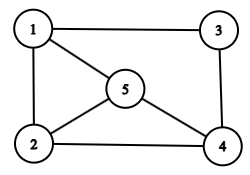
\includegraphics[width=\textwidth]{images/graph_cropped.png}
        \caption{Un graf G}
        \label{fig:graf}
    \end{minipage}\hfill
    \begin{minipage}{0.45\textwidth}
        \centering
        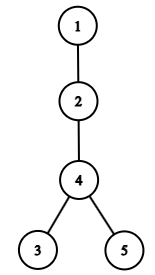
\includegraphics[width=\textwidth]{images/DFS_tree_cropped.png}
        \caption{Arborele traversării DFS, pornind din nodul 1}
        \label{fig:arbore}
    \end{minipage}
\end{figure}

{\fontsize{14}{16}\selectfont

Fie G, graful din figura \ref{fig:graf} si T, arborele din figura \ref{fig:arbore}. Pentru a forma in arborele T circuitul 1-2-5-1 din G, ar trebui sa introducem atat muchia 1-5, cat si 2-5. Insa, conform enuntului, $C_{xy}$ reprezinta arborele T, la care se adauga o singura muchie din G. Astfel, am gasit un contraexemplu in care nu putem forma toate circuitele din G adaugand doar cate o muchie, rezultand ca afirmatia este falsa. In plus, deoarece $\lbrace$ $C_{xy}$ : xy $\in$ E $\backslash$ E' $\rbrace$ nu conține toate circuitele din $G$, atunci nu vom fi niciodată siguri că circuitul de lungime minimă se poate afla prin prelucrarea unei traversări DFS a lui $G$.
}


\section*{\fontsize{20}{50}\selectfont Problema 3}
\subsection*{\fontsize{16}{30}\selectfont Subpunctul a}
{\fontsize{14}{16}\selectfont
Inainte de a incepe demonstratiile de la urmatoarele subpuncte, vom explica intregul algoritm.

In primul for al algoritmului, cozile de arce sunt initializate cu null.
Apoi, nodul "s" de start este plasat in multimea S a nodurilor vizitate, iar costul drumului minim si nodul anterior al sau sunt actualizate. Ultima instructiune din for plaseaza toate muchiile care ies din s in coada aferenta pretului sau.

Apoi, while-ul parcurge nodurile grafului pana cand toate sunt vizitate. Inainte de a incepe prelucrarea, functia Search() va fi apelata, functie care va returna muchia corespunzatoare celui mai scurt drum de la origine pana la capatul drept al muchiei. Apoi, capatul drept al muchiei returnate este marcat ca vizitat, ii este actualizat drumul minim si ii este actualizat nodul anterior. 

In final, algoritmul itereaza prin toate arcele care ies din j* si le plaseaza in coada corespunzatoare.
}
\subsubsection*{\fontsize{14}{20}\selectfont Subpunctul a1}
{\fontsize{14}{16}\selectfont
Este evident ca algoritmul va plasa nodurile in S in ordinea crescatoare a costurilor minime a drumurilor din s, deoarece atunci cand alege o muchie pe care sa isi continue exectuia, compara costurile drumurilor din s pana in capatul drept al muchiei, urmand sa il returneze pe cel mai mic. Deoarece nu exista costuri negative in digraf, drumurile create cu muchiile din cozi vor continua sa creasca in pret, deci nu va aparea in cozi niciodata o muchie cu un drum cu cost mai mic decat orice alt drum parcurs in trecut.
}

\subsubsection*{\fontsize{14}{20}\selectfont Subpunctul a2}
{\fontsize{14}{16}\selectfont

Deoarece algoritmul adauga arce in $L_h$ pe masura ce exploreaza nodurile, iar nodurile sunt alese in ordine crescatoare a costurilor $u_i$, daca $u_i$< $u_j$ atunci algoritmul a explorat nodul i inainte de nodul j si, implicit, a adaugat arcele ce ies din i (printre care si ij) inaintea celor care ies din i' (printre care si i'j'). Astfel, daca doua arce ij si i'j' apartin aceleiasi cozi si $u_i$< $u_j$, ij apare inaintea lui i'j' in $L_h$.

}

\subsubsection*{\fontsize{14}{20}\selectfont Subpunctul a3}
{\fontsize{14}{16}\selectfont
Luand conditiile pe ordine, putem demonstra de ce structura cozii Lh ramane aceeasi pe toata durata algoritmului

$\lbrace$ i $\in$ S $\rbrace$ : Atunci cand adaugam arce in coada Lh, iteram prin vecinii lui j* si punem in coada arcele corespunzatoare nodurilor neexplorate. Deoarece adaugarea arcelor in coada se face dupa ce j* este marcat ca un nod vizitat, iar nodurile nu sunt scoase niciodata din multimea nodurilor vizitate, aceasta conditie este indeplinita.

$\lbrace$ j $\notin$ S $\rbrace$ : Inainte de apelarea functiei Search(), conditia este indeplinita deoarece adaugam in cozi doar nodurile care $\notin$ S. In timpul apelarii, daca capatul drept al oricarii arc dintr-o coada este vizitat, atunci acesta este eliminat din coada. Astfel, dupa apelare nu va mai exista in coada nici un arc cu capatul drept explorat, respectandu-se conditia.

$a_{ij}$ = $\gamma_h$ : Aceasta conditie este permanent indeplinita pentru ca, inainte de a adauga un arc in coada este verificata.

Astfel, deoarece toate cele 3 conditii sunt indeplinite, putem spune ca $\lbrace$ ij : i $\in$ S, j $\notin$ S, $a_{ij}$ = $\gamma_h$ $\rbrace$ $\subseteq$ $L_h$ inainte si dupa fiecare iteratie a buclei while.

}

\subsubsection*{\fontsize{14}{20}\selectfont Subpunctul a4}
{\fontsize{14}{16}\selectfont

La început, cozile $L_h$ sunt inițializate cu valori nule și se adaugă doar muchiile vecine nodului de start. Este important de observat că în această fază doar nodul de start se află în mulțimea S a nodurilor vizitate. După intrarea în bucla while, variabila ij* primește rezultatul funcției Search(), care caută în toate muchiile din $L_h$ și returnează muchia xy aferenta drumului cu cost minim, unde x$\in$S și y$\notin$S. Abia după ce ij* este selectat, nodul j* este adăugat în S, iar muchiile incidente cu acesta sunt adăugate în $L_h$, fără ca celelalte capete ale acestor muchii să fie incluse în S. Deci, oricum am alege muchia ij*, aceasta va reprezenta drumul cu cel mai mic cost dintre toate celelalte drumuri pe care le putem forma cu muchiile din cozi.

}

\subsection*{\fontsize{16}{30}\selectfont Subpunctul b}
{\fontsize{14}{16}\selectfont
Primul for al algoritmului are o complexitate O(p). Urmatorul for, care itereaza prin vecinii lui i se face in timp constant. While-ul principal va itera prin toate nodurile digrafului, adica va avea complexitatea O(n), si va apela functia Search() la fiecare pas.

Functia Search() verifica fiecare arc din cozi. In cel mai rau caz, va verifica toate arcele la fiecare apelare, adica va avea complexitatea O(m).

In final, complexitatea algoritmului va fi  \\ \centerline {O(p) + O(n) * O (m) = O(n*m).}
}

\section*{\fontsize{20}{50}\selectfont Problema 4}

\subsection*{\fontsize{16}{30}\selectfont Subpunctul a}
{\fontsize{14}{16}\selectfont
$G'$ este obținut prin eliminarea de muchii din $G$, pe baza unei condiții descrise în algoritmul dat, iar $G$ nu are circuite de lungime $\le 4$. Așadar, $G'$ nu poate avea nici el circuite de lungime $\le 4$ întrucât eliminarea de muchii nu poate genera circuite, ci poate doar menține sau micșora numărul de circuite din acel graf.}

\subsection*{\fontsize{16}{30}\selectfont Subpunctul b}
{\fontsize{14}{16}\selectfont
Presupunem prin reducere la absurd că $V_{u,1} \cap V_{u,2} \neq \emptyset$. Înseamna că $\exists x$ astfel încât $x \in V_{u,1}$ și $x \in V_{u,2}$. Pentru că $x \in V_{u,2}$, trebuie să existe $v \in V_{u,1}, v \ne x$ astfel încât $v$ și $x$ să fie adiacente. Dar pentru că $x,v \in V_{u,1}$, înseamnă că $u$ este adiacent cu $x$ și $v$. Astfel, se formează un circuit de lungime 3 ($u \rightarrow v \rightarrow x$), ceea ce contrazice faptul că $G'$ nu conține circuite de lungime $\le 4$. Deci, $V_{u,1} \cap V_{u,2} = \emptyset$.}
\\
{\fontsize{14}{16}\selectfont
Dacă oricare două noduri din $V_{u,1}$ sunt adiacente, se formează un circuit de lungime 3, deoarece $u$ este adiacent cu fiecare dintre nodurile din $V_{u,1}$, inclusiv cele două. Acest lucru nu este posibil deoarece $G$ și $G'$ nu conțin circuite de lungime $\le 4$.}

\end{document}